\documentclass[12pt]{article}
\textwidth 16.5cm
\textheight 23.5cm
\oddsidemargin 0pt
\topmargin -2cm
% \usepackage{epsf}

% Writing maths
\usepackage{
    amsmath, % aligns, equations, etc.
    amsfonts, % blackboard bold, etc.
    bbm, % blackboard bold for numbers.
}

% Figures
\usepackage{graphicx}

% References 
\usepackage{natbib}
\bibliographystyle{natbib}
\setcitestyle{authoryear, open={(},close={)}}

% Inline comments from Jacob and Bella
\usepackage{xcolor}
\usepackage[draft,inline,nomargin,index]{fixme}
\fxsetup{theme=color,mode=multiuser}
\FXRegisterAuthor{jb}{ajb}{\color{blue} JB}
\FXRegisterAuthor{bd}{abd}{\color{red} BD}

\title{Simulations of Immigration Queues at Edinburgh Airport: Report}
 \author{Isabella Deustch, Jacob R. Bradley
 \\ \emph{School of Mathematics, University of Edinburgh}}

\begin{document}
\maketitle

\section{Introduction}
This document contains the results of Jacob and Bella's project to submit to the modelling competition. It should be ten pages or fewer. \jbnote{including references?}
\section{Methods}
\section{Results}

\begin{figure}[htbp]
    \centering
    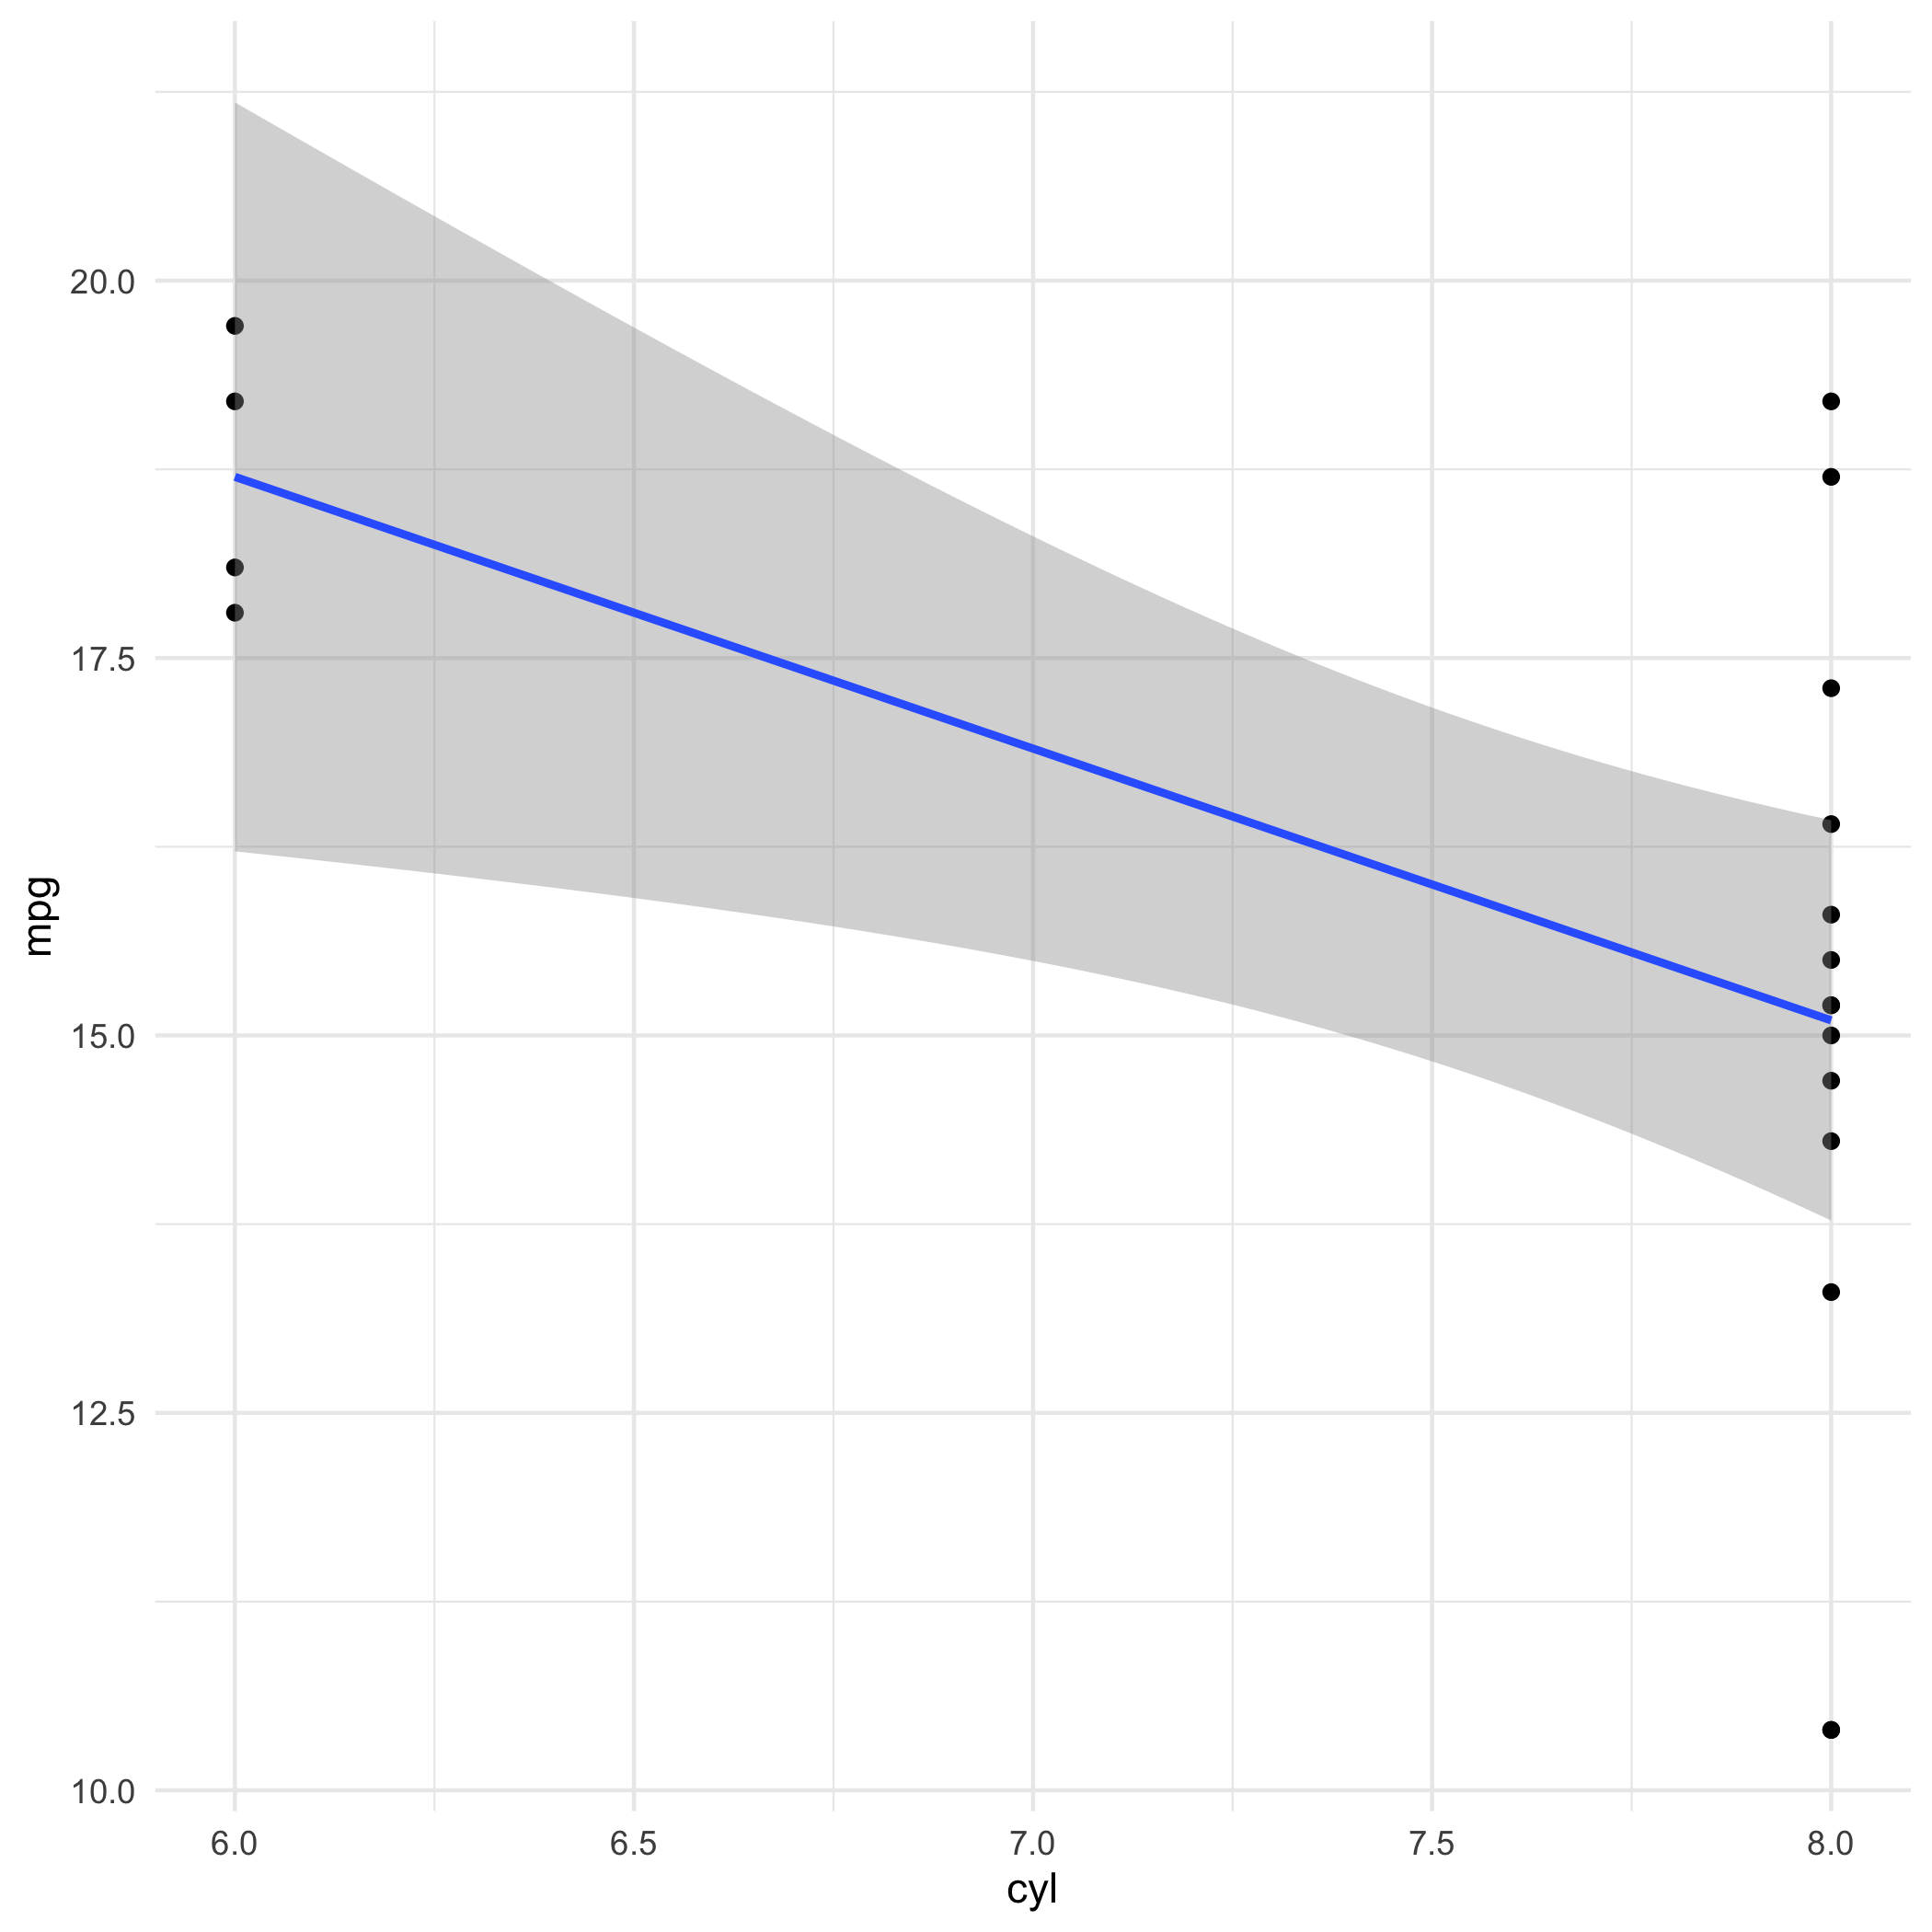
\includegraphics[width=4in]{figures/mt_cars_summary.png}
    \caption{Example figure generated from mtcars workflow.}
    \label{fig:mtcars}
\end{figure}

\section{Discussion}
\section{Conclusion}
% \bibliography{references.bib}
\end{document}